\documentclass[11pt,a4paper]{article}
\usepackage{hyperref}
\usepackage{graphicx}

\begin{document}
\title{Treacherous Talks -
  Sprint 4: ``Find the Limits of Real Games''}
\date{\today}
\author{Spokesperson: stephan.brandauer@gmail.com}
\maketitle

\section{The Sprint}
\subsection{Plan ..}
The main focus of this sprint was to load test our system and find out where
our bottlenecks are. This also made it necessary (or very helpful) to further
improve our build system and especially to create a centralised way to start
and connect a whole cluster on several machines: the {\tt cluster\_manager}. \\
We also worked on fault tolerance of our backends: the ultimate goal here is
to handle the breakdown of servers gracefully: requiring users logged in on the
broken server to re-login and restarting games that were running on a different
server. We also scheduled much work on the in-game and off-game messaging system.

\subsection{.. and Reality}
We managed to fulfill the sprint goal and even pulled in more stories from
the back log, handling some features regarding the ``operator''-role:
dynamically adding and removing servers to our backend-cluster. \\
The benchmarks immediately highlighted some small bugs with big influences:
an unreasonable hunger for memory and the unnecessary allocation of ets-tables
that made us hit an internal limit on their numbers quickly. \\ Both of these
bugs where identified and resolved quickly. \\
More worrying (because it is unresolved) though is the fact that our system exhibits throughput
degradation under load; one of sprint 5's goals is to fix that problem. \\
We also evaluated our system in terms of scalability and are quite happy with
these results, although we do not think that what we have is enough.

\begin{figure}[h]
 \centering
 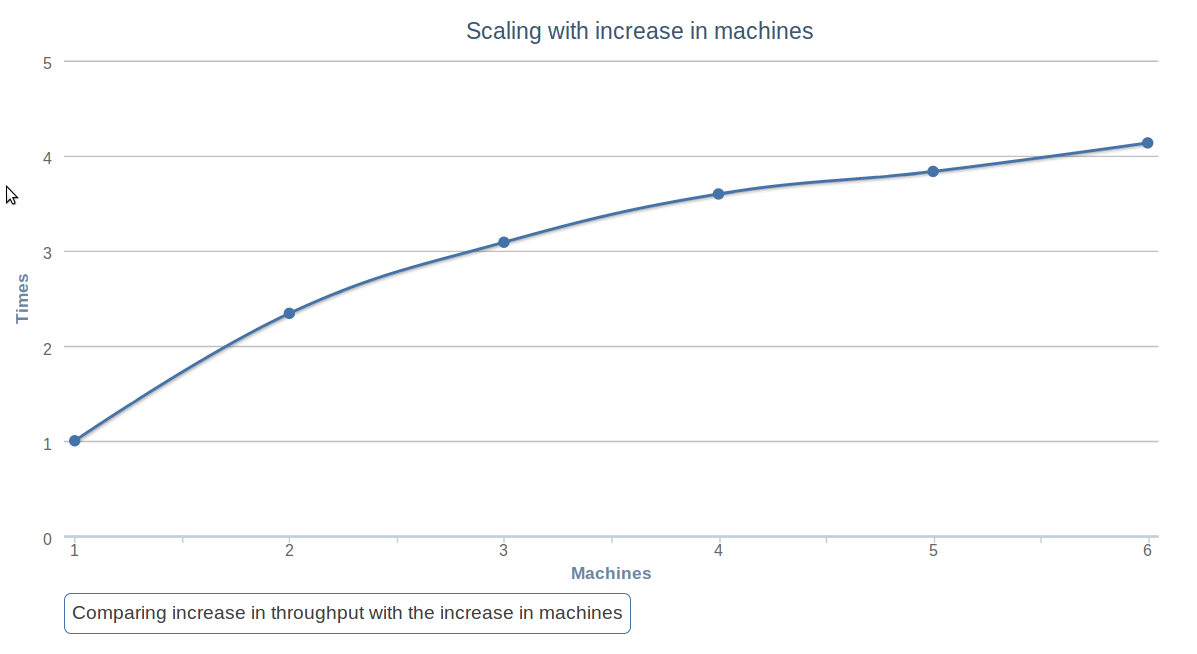
\includegraphics[width=10cm,keepaspectratio=true]{./scale.png}
 % scale.png: 1197x654 pixel, 72dpi, 42.22x23.07 cm, bb=0 0 1197 654
 \caption{The speedup from 1 to 6 servers, no frontends included}
 \label{fig:speedup}
\end{figure}

\newpage

\subsection{The Stories}
\begin{itemize}
\item Choose Open Source license to license our code: done (MIT license)
\item Setup smtp interface tests: done
\item Game testing: done
\item Improve releases: done
\item Game app refactoring: done
\item A user should be able to search for games based on properties: done
\item A user should be able to communicate with other players outside the game: done
\item A user should be able to communicate with the other players in a game according to the type of press selected: done
\item Setup load testing: done
\item Set up fault tolerance tests: done
\item An operator should be able to add servers to the system without reconfiguration of existing servers: done
\item An operator should be able to remove servers from the system without reconfiguration of existing servers: done
\end{itemize}

\end{document}
